\subsection{半直积}

设 \(\mathfrak{a}\) 和 \(\mathfrak{b}\) 是 \(\mathbf{K}\) 上的两个李代数。构造 \(\mathfrak{b}\) 的所有由 \(\mathfrak{a}\) 作的扩张并不容易。但我们将相当简单地描述 \(\mathfrak{b}\) 的所有由 \(\mathfrak{a}\) 作的非本质扩张。

设 \(g\) 是 \(b\) 的 \(a\)-非本质扩张。我们把 \(a\) 与 \(g\) 的一个理想相同，把 \(b\) 与 \(g\) 中补 \(a\) 的一个子代数相同，并把模 \(g\) 与模 \(a \times b\) 相同。对所有 \(b \in b\)，令 \(\phi_b\) 为 \(a\) 上 \(ad_g b\) 的限制；它是 \(a\) 的导子，而映射 \(b \mapsto \phi_b\) 是从 \(b\) 到 \(a\) 的导子李代数的同态。另一方面，对 \(a, a'\) 中的 \(a\) 和 \(b, b'\) 中的 \(b\)，有：

\[
\begin{array}{r l} {[ (a, b), (a ^ {\prime}, b ^ {\prime}) ]} & {= [ a + b, a ^ {\prime} + b ^ {\prime} ]} \\ & {= [ a, a ^ {\prime} ] + [ a, b ^ {\prime} ] + [ b, a ^ {\prime} ] + [ b, b ^ {\prime} ]} \\ & {= ([ a, a ^ {\prime} ] + \phi_ {b} a ^ {\prime} - \phi_ {b ^ {\prime}} a, [ b, b ^ {\prime} ]).} \end{array}\tag{6}
\]

反之，设 \(\mathfrak{a}\) 和 \(\mathfrak{b}\) 是 \(\mathbf{K}\) 上的李代数，\(b \mapsto \phi_b\) 是从 \(\mathfrak{b}\) 到 \(\mathfrak{a}\) 的导子李代数的同态。在 \(\mathfrak{g}\)（K-模 \(\mathfrak{a}\) 与 \(\mathfrak{b}\) 的积）上，我们如下定义两个元素的括号：

\[
[ (a, b), (a ^ {\prime}, b ^ {\prime}) ] = ([ a, a ^ {\prime} ] + \phi_ {b} a ^ {\prime} - \phi_ {b ^ {\prime}} a, [ b, b ^ {\prime} ])
\]

对所有 \(a, a'\) 属于 \(\mathfrak{a}, b, b'\) 属于 \(\mathfrak{b}\)。立即可见，此括号是关于 \((a, b), (a', b')\) 的交错双线性函数；我们说明，对于 \((a, b), (a', b'), (a'', b'')\) 这三个 \(\mathfrak{a} \times \mathfrak{b}\) 中的元素，有：

\[
\begin{array}{r l} {[ (a, b), [ (a ^ {\prime}, b ^ {\prime}), (a ^ {\prime \prime}, b ^ {\prime \prime}) ] ] + [ (a ^ {\prime}, b ^ {\prime}), [ (a ^ {\prime \prime}, b ^ {\prime \prime}), (a, b) ] ]} & \\ {+ [ (a ^ {\prime \prime}, b ^ {\prime \prime}), [ (a, b), (a ^ {\prime}, b ^ {\prime}) ] ] = 0.} \end{array}\tag{7}
\]

由于 (7) 的左端是关于 \((a, b)\)、\((a', b')\)、\((a'', b'')\) 的交错三线性函数，只需在这组元素取下列形式之一时验证：

\[
(a, 0), (a ^ {\prime}, 0), (a ^ {\prime \prime}, 0)\tag{8}
\]

\[
(a, 0), (a ^ {\prime}, 0), (0, b ^ {\prime \prime})\tag{9}
\]

\[
(a, 0), (0, b ^ {\prime}), (0, b ^ {\prime \prime})\tag{10}
\]

\[
(0, b), (0, b ^ {\prime}), (0, b ^ {\prime \prime})\tag{11}
\]

在情形 (8) 和 (11) 中，关系 (7) 立即由 a 和 b 中的 Jacobi 恒等式得到。在情形 (9) 中，有

\[
\begin{array}{l} [ (a, 0), [ (a ^ {\prime}, 0), (0, b ^ {\prime \prime}) ] ] = [ (a, 0), (- \phi_ {b ^ {\prime \prime}} a ^ {\prime}, 0) ] = (- [ a, \phi_ {b ^ {\prime \prime}} a ^ {\prime} ], 0) \\ {} [ (a ^ {\prime}, 0), [ (0, b ^ {\prime \prime}), (a, 0) ] ] = [ (a ^ {\prime}, 0), (\phi_ {b ^ {\prime \prime}} a, 0) ] = ([ a ^ {\prime}, \phi_ {b ^ {\prime \prime}} a ], 0) \\ {} [ (0, b ^ {\prime \prime}), [ (a, 0), (a ^ {\prime}, 0) ] ] = [ (0, b ^ {\prime \prime}), ([ a, a ^ {\prime} ], 0) ] = (\phi_ {b ^ {\prime \prime}} ([ a, a ^ {\prime} ]), 0) \end{array}
\]

关系 (7) 由下式得到：

\[
\phi_ {b ^ {\prime \prime}} ([ a, a ^ {\prime} ]) = [ \phi_ {b ^ {\prime \prime}} a, a ^ {\prime} ] + [ a, \phi_ {b ^ {\prime \prime}} a ^ {\prime} ].
\]

在情形 (10) 中，有：

\[
[ (a, 0), [ (0, b ^ {\prime}), (0, b ^ {\prime \prime}) ] ] = [ (a, 0), (0, [ b ^ {\prime}, b ^ {\prime \prime} ]) ] = (- \phi_ {[ b ^ {\prime}, b ^ {\prime \prime} ]} a, 0)
\]

\[
[ (0, b ^ {\prime}), [ (0, b ^ {\prime \prime}), (a, 0) ] ] = [ (0, b ^ {\prime}), (\phi_ {b ^ {\prime \prime}} a, 0) ] = (\phi_ {b ^ {\prime}} \phi_ {b ^ {\prime \prime}} a, 0)
\]

\[
[ (0, b ^ {\prime \prime}), [ (a, 0), (0, b ^ {\prime}) ] ] = [ (0, b ^ {\prime \prime}), (- \phi_ {b ^ {\prime}} a, 0) ] = (- \phi_ {b ^ {\prime \prime}} \phi_ {b ^ {\prime}} a, 0)
\]

关系 (7) 由下式得到：

\[
\phi_ {[ b ^ {\prime}, b ^ {\prime \prime} ]} = \phi_ {b ^ {\prime}} \phi_ {b ^ {\prime \prime}} - \phi_ {b ^ {\prime \prime}} \phi_ {b ^ {\prime}}.
\]

于是，g 上定义了李代数结构。从 g 到 b 的映射 \((a, b) \mapsto b\) 是同态 \(\mu\)，其核 n 是 g 中形如 \((a, 0)\) 的元素组成的理想。映射 \(a \mapsto (a, 0)\) 是将 a 同构到 n 上的同构 \(\lambda\)。因此：

\[
a \xrightarrow {\lambda} g \xrightarrow {\mu} b\tag{12}
\]

这是一个核为 n 的由 a 扩张 b 的扩张，称为由 a、b、\(\phi\) 典范定义的扩张。映射 \(b \mapsto (0, b)\) 是将 b 同构到 g 的一个补 n 的子代数上的同构 v；因此该扩张是非本质的。

若在识别 \(a\) 与 \(n\) 时使用 \(\lambda\)，并在识别 \(b\) 与 \(v(b)\) 时使用 \(v\)，则对 \(a \in a\) 和 \(b \in b\)：

\[
(\mathrm{ad} b). a = [ (0, b), (a, 0) ] = (\phi_ {b} a, 0) = \phi_ {b} a.
\]

当 \(\phi = 0\) 时，\(\mathfrak{g}\) 是 \(\mathfrak{b}\) 与 \(\mathfrak{a}\) 的积李代数。一般情形下，\(\mathfrak{g}\) 称为 \(\mathfrak{b}\) 由 \(\mathfrak{a}\) 作的半直积（对应于 \(b \mapsto \phi_b\) 从 \(\mathfrak{b}\) 到 \(\mathfrak{a}\) 的导子李代数的同态）。

因此我们得到了下述命题：

命题 7. 设 a 和 b 是 K 上的两个李代数，

\[
a \xrightarrow {\lambda} g \xrightarrow {\mu} b
\]

是由 a 扩张 b 的非本质扩张，v 是将 b 同构到 g 的一个子代数上的同构，且 \(\mu \circ v\) 是 b 的恒等自同构；\(\phi\) 是相应的从 b 到 a 的导子李代数的同态。设

\[
a \xrightarrow {\lambda_ {0}} g _ {0} \xrightarrow {\mu_ {0}} b
\]

是由 a 扩张的 \(\mathfrak{b}\)、由 \(\phi\) 典范定义的非本质扩张。则映射 \((a, b) \mapsto \lambda(a) + v(b)\) 是同构 \(f\)，从 \(\mathfrak{g}_0\) 到 \(\mathfrak{g}\)，且下图

\pandocbounded{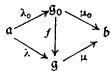
\includegraphics[keepaspectratio]{images/part001_108a7b03.jpg}}

是交换的，因此两个扩张等价。

例 1. 设 g 是 K 上的李代数，D 是 g 的导子。令 h 为交换李代数 K。映射 \(\lambda \mapsto \lambda D (\lambda \in \mathbf{K})\) 是从 h 到 g 的导子李代数的同态。我们构造 h 由 g 作的相应半直积 t。令 \(x_0\) 为 t 的元素 (0, 1)。对所有 \(x \in g\)，有 Dx = [x₀, x]。

例 2. 设 g 是 K 上的李代数，M 是 K-模，\(\rho\) 是从 g 到 gl(M) 的同态。若把 M 视为交换李代数，则 M 的导子李代数就是 gl(M)。因此，我们可以构造对应于 \(\rho\) 的 M 由 g 作的半直积 h。

特别地，令 \(\mathfrak{g} = \mathfrak{gl}(\mathbf{M})\)，\(\rho\) 为 \(\mathfrak{gl}(\mathbf{M})\) 的恒等映射。于是，\(\mathfrak{g}\) 由 \(\mathbf{M}\) 作的半直积记作 \(\mathfrak{af}(\mathbf{M})\)（或记作 \(\mathfrak{af}(n,\mathbf{K})\)，当 \(\mathbf{M} = \mathbf{K}^{n}\) 时）。\(\mathfrak{af}(\mathbf{M})\) 的元素是有序对 \((m,u)\)，其中 \(m\in \mathbf{M}\)、\(u\in \mathfrak{gl}(\mathbf{M})\)；括号定义为

\[
[ (m, u), (m ^ {\prime}, u ^ {\prime}) ] = (u (m ^ {\prime}) - u ^ {\prime} (m), [ u, u ^ {\prime} ]).
\]

*当 M 是 R 上的有限维向量空间时，\(\mathfrak{af}(M)\) 自然地与 M 的仿射群的李代数相同。*

设 \(t\) 是 \(K\) 上的李代数。线性映射 \(\theta\) 从 \(t\) 到 \(\mathfrak{af}(M)\) 可写成 \(x \mapsto ((\zeta(x), \eta(x))\)，其中 \(\zeta\) 是从 \(t\) 到 \(M\) 的线性映射，\(\eta\) 是从 \(t\) 到 \(\mathfrak{gl}(M)\) 的线性映射。我们考察 \(\zeta\) 和 \(\eta\) 为使 \(\theta\) 成为同态必须满足的条件。对 \(x \in t, y \in t\)，必须有

\[
\theta ([ x, y ]) = [ \theta (x), \theta (y) ]
\]

即

\[
\begin{array}{r l} (\zeta ([ x, y ]), \eta ([ x, y ])) & = [ (\zeta (x), \eta (x)), (\zeta (y), \eta (y)) ] \\ & = (\eta (x). \zeta (y) - \eta (y). \zeta (x), [ \eta (x), \eta (y) ]). \end{array}
\]

因此，\(\theta\) 是从 \(t\) 到 \(\mathfrak{af}(M)\) 的同态的充要条件是：\(\eta\) 是从 \(t\) 到 \(\mathfrak{gl}(M)\) 的同态，且 \(\zeta\) 满足关系式：

\[
\zeta ([ x, y ]) = \eta (x). \zeta (y) - \eta (y). \zeta (x).\tag{13}
\]

令 \(\mathbf{N}\) 为 \(\mathbf{K}\)-模 \(\mathbf{M} \times \mathbf{K}\)。取 \(t\) 为 \(\mathfrak{gl}(\mathbf{N})\) 的子代数，由 \(w \in \mathfrak{gl}(\mathbf{N})\) 且满足 \(w(\mathbf{N}) \subset \mathbf{M}\) 的元素组成。对所有 \(w \in t\)，令 \(\eta(w) \in \mathfrak{gl}(\mathbf{M})\) 为 \(w\) 在 \(\mathbf{M}\) 上的限制，并令 \(\zeta(w) = w(0,1) \in \mathbf{M}\)。对 \(w_1 \in t, w_2 \in t\)，

\[
\zeta ([ w _ {1}, w _ {2} ]) = w _ {1} (\zeta (w _ {2})) - w _ {2} (\zeta (w _ {1})) = \eta (w _ {1}). \zeta (w _ {2}) - \eta (w _ {2}). \zeta (w _ {1}).
\]

因此映射 \(w \mapsto (\zeta(w), \eta(w))\) 是同态 \(\theta\)，它从 \(t\) 到 \(\mathfrak{af}(\mathbf{M})\)。显然 \(\theta\) 是双射。令 \(\phi = \theta^{-1}\)。若 \((m, u) \in \mathfrak{af}(\mathbf{M})\)，则 \(\phi(m, u)\) 是元素 \(w\)，它是 \(t\) 中由下式定义的：

\[
w (m ^ {\prime}, \lambda) = (u (m ^ {\prime}) + \lambda m, 0).
\]

\(\mathfrak{af}(\mathbf{M})\) 常被认作子代数 \(\mathfrak{t}\)，它属于 \(\mathfrak{gl}(\mathbf{N})\)，对应的同构为 \(\phi\)。

*当 M 是 \(\mathbf{R}\) 上的有限维向量空间时，同态 \(\phi\) 从 \(\mathfrak{af}(M)\) 到 \(\mathfrak{gl}(N)\)，对应于 M 的仿射群 A 到同态 \(\psi\)，它映到 \(\mathbf{GL}(N)\)；若 \(a \in A\)，则 \(\psi(a)\) 是唯一元素 \(g\)，它属于 \(\mathbf{GL}(N)\) 且满足 \(g(m, 1) = (a(m), 1)\) 对所有 \(m \in M\) 成立。此同态是单射，而 \(\psi(A)\) 是 N 的所有平行于 M 的线性簇均保持不变的自同构组成的集合。*

